%!TEX root = ../main.tex
%%%%%%%%%%%%%%%%%%%%%%%%%%%%%%%%%%
% Links:
%
% Difficulty:
% Companies: 
%%%%%%%%%%%%%%%%%%%%%%%%%%%%%%%%%%


%\begin{figure}
%	\centering
%	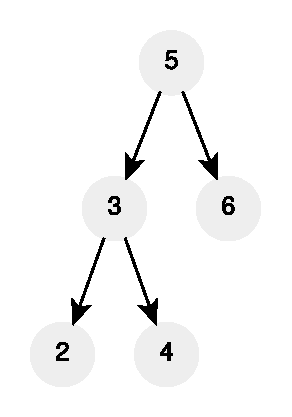
\includegraphics[width=\textwidth]{sources/allocate_books/images/example1}
%	\caption[Sample short cpation]{Sample Caption}.
%	\label{fig:allocate_books:example1}
%\end{figure}

\chapter{Assign books to students}
\label{ch:allocate_books}
\section*{Introduction}

\section{Problem statement}
\begin{exercise}
\label{example:allocate_books:exercice1}
Given an array of integers A of size N and an integer B.

College library has N bags,the ith book has A[i] number of pages.

You have to allocate books to B number of students so that maximum number of pages alloted to a student is minimum.

A book will be allocated to exactly one student.
Each student has to be allocated at least one book.
Allotment should be in contiguous order, for example: A student cannot be allocated book 1 and book 3, skipping book 2.
Calculate and return that minimum possible number.



Input Format

The first argument given is the integer array A.
The second argument given is the integer B.
Output Format

Return that minimum possible number
Constraints




	%example1
	\begin{example}
		\label{example:allocate_books:example1}
		\hfill \\
		
Input 1:
A = [12, 34, 67, 90]
B = 2
Output 1:
113
Explanation 1:
There are 2 number of students. Books can be distributed in following fashion : 
	1) [12] and [34, 67, 90]
	Max number of pages is allocated to student 2 with 34 + 67 + 90 = 191 pages
	2) [12, 34] and [67, 90]
	Max number of pages is allocated to student 2 with 67 + 90 = 157 pages 
	3) [12, 34, 67] and [90]
	Max number of pages is allocated to student 1 with 12 + 34 + 67 = 113 pages

	Of the 3 cases, Option 3 has the minimum pages = 113.
		
	\end{example}

	%example2
	\begin{example}
		\label{example:allocate_books:example2}
		\hfill \\
    A = [5, 17, 100, 11]
    B = 4
Output 2:
    100
	\end{example}


\end{exercise}

\section{Clarification Questions}

\begin{QandA}
	\item 
	\begin{answered}
		\textit{NOTE: Return -1 if a valid assignment is not possible.
		}
	\end{answered}
	
\end{QandA}

\section{Discussion}
\label{allocate_books:sec:discussion}
Solution strategy:
imagine you limit the numnber of pages to X per student. How many student you need to allocate all books?
Find the smallest X such that the number of students is exactly B.

\subsection{Brute-force}
\label{allocate_books:sec:bruteforce}

\begin{minipage}{\linewidth}
	\lstinputlisting[language=c++, caption={Sample Caption},label=list:allocate_books]{sources/allocate_books/allocate_books_solution1.cpp}
\end{minipage}

